\documentclass[12pt,a4paper,oneside,ngerman]{article} 
\usepackage[left=3cm,right=3cm,top=2.5cm]{geometry} % Groesse der Seitenraender definieren
\usepackage[utf8]{inputenc} % utf8 encoding
\usepackage{hyperref}
\usepackage{ngerman}[babel]
\usepackage{graphicx}
\usepackage{tikz} % Automaten, Graphen, ... zeichnen
\usepackage{tikz-qtree} % Paket fuer Tikz Graphen-Baeume
\usetikzlibrary{arrows,shapes,automata} % Bestimmte tikz-Befehle benutzen
\usepackage{amsmath,amssymb} % Mathe-Formeln und -Ausdruecke
\usepackage{listings} % Code-Ausschnitte einbinden
\usepackage{xcolor} % Eigene Farben definieren
\usepackage{colortbl} % Farben verwenden in Tabellen
\usepackage{wrapfig} % Bilder von Text umfliessen lassen
\usepackage{multicol} % Mehrspaltigen Text schreiben
\usepackage{stmaryrd} % Fuer Symbole wie zu Beispiel Widerspruchspfeil
\usepackage{caption}
\usepackage{totpages}

\usepackage{circuitikz}
\usepackage{amsmath}
\usepackage{graphicx}
\usepackage{subfigure}
\usepackage{tikz}
\usepackage{float}

\lstset{language=Java,
basicstyle=\small \ttfamily,
keywordstyle=\color{javapurple}\bfseries,
stringstyle=\color{javared},
commentstyle=\color{javagreen},
morecomment=[s][\color{javadocblue}]{/**}{*/},
numbers=left,
numberstyle=\tiny\color{black},
stepnumber=1,
numbersep=10pt,
tabsize=1,
showspaces=false,
showstringspaces=false,
breaklines=true}
\lstset{literate=%
  {Ö}{{\"O}}1
  {Ä}{{\"A}}1
  {Ü}{{\"U}}1
  {ß}{{\ss}}1
  {ü}{{\"u}}1
  {ä}{{\"a}}1
  {ö}{{\"o}}1
}

% Beliebige RGB Farben definieren:
\definecolor{gold}{rgb}{0.83, 0.69, 0.15}
\definecolor{magenta}{rgb}{0.79, 0.08, 0.48}
\definecolor{javared}{rgb}{0.6,0,0} % for strings
\definecolor{javagreen}{rgb}{0.25,0.5,0.35} % comments
\definecolor{javapurple}{rgb}{0.5,0,0.35} % keywords
\definecolor{javadocblue}{rgb}{0.25,0.35,0.75} % javadoc

% Beliebige RGB Farben definieren:
\definecolor{gold}{rgb}{0.83, 0.69, 0.15}
\definecolor{magenta}{rgb}{0.79, 0.08, 0.48}

% Titel in Kopfzeilen
\usepackage{fancyhdr}
\pagestyle{fancy}
\fancyhf{}
\setlength{\headheight}{20pt}

% Seitenumbrueche werden nicht mehr eingerueckt
\setlength{\parindent}{0em}


% % % % % % % % % % % % % % % % % % % % % % % % % % % % % % 
%Variablen
% % % % % % % % % % % % % % % % % % % % % % % % % % % % % % 
\newcommand{\fach}{Objektorientierte Modellierung und Programmierung}
\newcommand{\dokumentenTitel}{Abgabe Uebungsblatt Nr.03}
\newcommand{\Abgabe}{12.05.2020, 12:00 Uhr}
\newcommand{\memberOne}{Marius Birk}
\newcommand{\memberTwo}{Pieter Vogt}


\newcommand{\tutor}{ Florian Brandt }
% % % % % % % % % % % % % % % % % % % % % % % % % % % % % 

% Kopfzeile auf jeder Seite:
\fancyhead[R]{\dokumentenTitel} % Dokument-Titel
\fancyhead[C]{}
\fancyhead[L]{\memberOne, \memberTwo} % Autorennamen
\renewcommand{\headrulewidth}{0.4pt} %obere Trennlinie

% Fußzeile auf jeder Seite:
\fancyfoot[C]{Seite \thepage \ von \ref{TotPages}} %Seitennummer
\renewcommand{\footrulewidth}{0.4pt} %untere Trennlinie

% Nun beginnt das eigentliche Dokument
\begin{document}
	\thispagestyle{plain} % Keine Kopfzeile auf erster Seite, aber Seitenzahl wird angezeigt
	
	\begin{multicols}{2} % Beginnt zweispaltigen Text fuer Header auf erster Seite
		\hspace{-1cm} % Linken Header-Teil 1cm nach links schieben.
		% Tabelle fuer linke Seite vom Header der ersten Seite
		\begin{tabular}{ll} % Mit l werden die Eintraege linksbuendig
			Autoren: & \memberOne \\ % Zwischen jeder Spalte ein & einfuegen
			& \memberTwo \\
% beendet eine Tabellenzeile 
			Tutor: & \tutor \\  
		\end{tabular}
		
		\columnbreak % Nun beginnt die rechte Seite des Headers
		\hspace{-1cm} % Rechten Header-Teil 1cm nach links schieben.
		% Tabelle fuer rechte Seite vom Header der ersten Seite
		\begin{tabular}{ll} % p{1cm} bewirkt, dass die rechte Spalte 6cm breit ist.
			Abgabe: & \Abgabe \\ % Zwischen jeder Spalte ein & einfuege
			Smileys: &  
			%Mit diesem Befehl wird die Zeilenhoehe der folgenden Tabelle um 20% erhoeht.   
			\renewcommand{\arraystretch}{1.2} 
			% Nun kommt eine innere Tabelle in der aeusseren Tabelle, mit der eine Punktetabelle fuer den Tutor erstellt wird:  
			\begin{tabular}{|p{0.8cm}|p{0.8cm}|p{0.8cm}|}
				\hline A1 & A2 & $\sum\limits^{ }$ \\ \hline
				& & \\ \hline    
			\end{tabular} \\
		\end{tabular}
		
	\end{multicols} % Beendet zweispaltigen Text
	
	\begin{center}
		\Large{\fach} \\
		\LARGE{\dokumentenTitel} \\
		\small
		$($Alle allgemeinen Definitionen aus der Vorlesung haben in diesem Dokument bestand, es sei den sie erhalten eine explizit andere Definition.$)$
	\end{center}
\section*{Aufgabe 1}
\subsection*{a)}
\begin{figure}[ht]
	\centering
  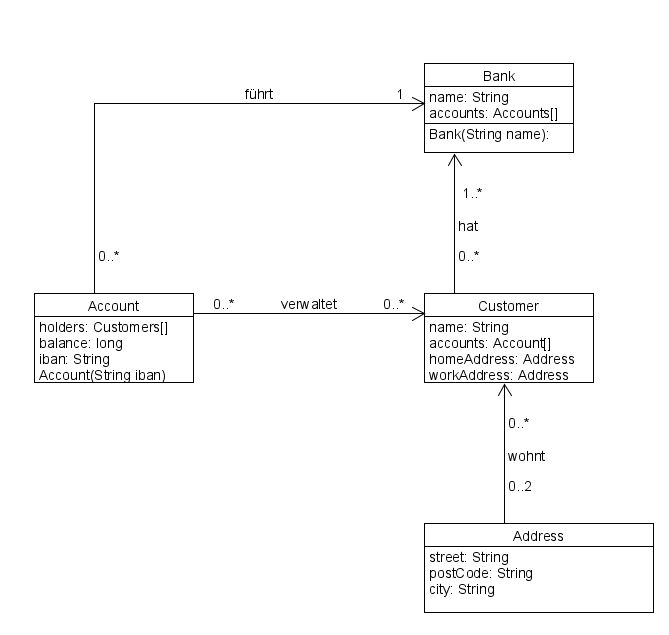
\includegraphics[width=\textwidth]{Von Marius/1_a_Klassendiagramm}
	\caption{Klassendiagramm}
\end{figure}
\subsection*{b)}
\begin{figure}[ht]
	\centering
  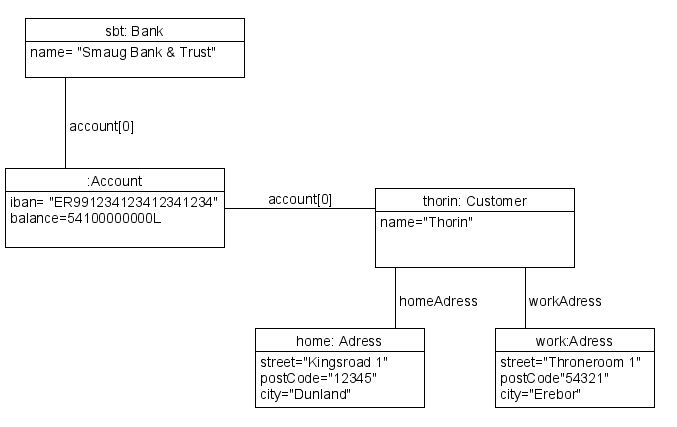
\includegraphics[width=\textwidth]{Von Marius/1_b_Objektdiagramm}
	\caption{Objektdiagramm}
\end{figure}

\subsection*{c)}

Account Klasse
\begin{lstlisting}
public class Account {
	
	private Customer[] holders;
	private long balance;
	private String iban;
	
	public Account(String iban) { this.iban = iban; }

	public Customer[] getHolders() { return holders; }

	public void setHolders(Customer[] holders) { this.holders = holders; }

	public long getBalance() { return balance; }

	public void setBalance(long balance) { this.balance = balance; }

	public String getIban() { return iban; }

}

\end{lstlisting}

Adress Klasse
\begin{lstlisting}
public class Address {
	
	private String street;
	private String postCode;
	private String city;

	public String getStreet() { return street; }
	
	public void setStreet(String street) { this.street = street; }
	
	public String getPostCode() { return postCode; }
	
	public void setPostCode(String postCode) { this.postCode = postCode; }
	
	public String getCity() { return city; }
	
	public void setCity(String city) { this.city = city; }

}
\end{lstlisting}

Bank Klasse
\begin{lstlisting}
public class Bank {
	
	private String name;
	private Account[] accounts;

	public Bank(String name) { this.name = name; }
	
	public String getName() { return name; }

	public void setName(String name) { this.name = name; }

	public Account[] getAccounts() { return accounts; }

	public void setAccounts(Account[] accounts) { this.accounts = accounts; }

}

\end{lstlisting}

Banking Klasse
\begin{lstlisting}
public class Banking {
	
	public static void main(String[] args) {
		Bank sbt = new Bank("Smaug Bank & Trust");
		sbt.setAccounts(new Account[1]);
		sbt.getAccounts()[0] = new Account("ER99123412341234123412");
		sbt.getAccounts()[0].setBalance(54100000000L);
		Customer thorin = new Customer();
		thorin.setAccounts(new Account[1]);
		thorin.getAccounts()[0] = sbt.getAccounts()[0];
		thorin.setName("Thorin");
		Address home = new Address();
		home.setStreet("Kingsroad 1");
		home.setPostCode("12345");
		home.setCity("Dunland");
		thorin.setHomeAddress(home);
		Address work = new Address();
		work.setStreet("Throneroom 1");
		work.setPostCode("54321");
		work.setCity("Erebor");
		thorin.setWorkAddress(work);
		sbt.getAccounts()[0].setHolders(new Customer[] { thorin });
	}

}

\end{lstlisting}

Customer Klasse
\begin{lstlisting}
public class Customer extends Person{
	private Account[] accounts;

	public Account[] getAccounts() { return accounts; }
	
	public void setAccounts(Account[] accounts) { this.accounts = accounts; }
}

\end{lstlisting}

FinancialAdvisor Klasse
\begin{lstlisting}
public class FinancialAdvisor extends Person{
    private Account[] supervised;
}

\end{lstlisting}

HomeAdress Klasse
\begin{lstlisting}
public class homeAddress extends Address{
    private String poBoxCode;
    private String poBoxCity;

    public String getPoBoxCode() {
        return poBoxCode;
    }

    public void setPoBoxCode(String poBoxCode) {
        this.poBoxCode = poBoxCode;
    }

    public String getPoBoxCity() {
        return poBoxCity;
    }

    public void setPoBoxCity(String poBoxCity) {
        this.poBoxCity = poBoxCity;
    }
}

\end{lstlisting}

Person Klasse
\begin{lstlisting}
public class Person {
    private String name;
    private Address homeAddress;
    private Address workAddress;

    public String getName() {
        return name;
    }

    public void setName(String name) {
        this.name = name;
    }

    public Address getHomeAddress() {
        return homeAddress;
    }

    public void setHomeAddress(Address homeAddress) {
        this.homeAddress = homeAddress;
    }

    public Address getWorkAddress() {
        return workAddress;
    }

    public void setWorkAddress(Address workAddress) {
        this.workAddress = workAddress;
    }
}

\end{lstlisting}

WorkAdress Klasse
\begin{lstlisting}
public class workAddress extends Address{
    private String companyName;

    public String getCompanyName() {
        return companyName;
    }

    public void setCompanyName(String companyName) {
        this.companyName = companyName;
    }
}
\end{lstlisting}

\section*{Aufgabe 2}
Die VersatileLinked List:
\begin{lstlisting}
public class VersatileLinkedList extends LinkedStringList {

   public void add(int i) {
      super.add(Integer.toString(i));
   }

   public void add(boolean b) {
      if (b == true) {
         super.add("yes");
      } else {
         super.add("no");
      }
   }

   public void add(LinkedStringList list) {
      for (int i = 0; i < list.size(); i++) {
         super.add(list.get(i));
      }
   }

   public void add(LinkedStringList list, int start, int end) {
      if (start > end || start < 0 || end > list.size()) {
         return;
      } else {
         for (int i = start; i < end; i++) {
            super.add(list.get(i));
         }
      }
   }

   public VersatileLinkedList reverse() {
      VersatileLinkedList temp = new VersatileLinkedList();
      for (int i = this.size() - 1; i >= 0; i--) {
         temp.add(this.get(i));
      }
      return temp;
   }

   public boolean equals(VersatileLinkedList list) {
      if (this.size() != list.size()) {
         return false;
      } else {
         for (int i = 0; i < this.size(); i++) {
            if (this.get(i).equals(list.get(i))) {
               i++;
            } else {
               return false;
            }
         }
         return true;
      }
   }

   public void print() {
      for (int i = 0; i < this.size(); i++) {
         System.out.println(this.get(i));
      }
   }
}

\end{lstlisting}
Die Main Methode zum testen:
\begin{lstlisting}
public class Main {
   public static void main(String[] args) {

      VersatileLinkedList ListA = new VersatileLinkedList();
      VersatileLinkedList ListB = new VersatileLinkedList();
      VersatileLinkedList ListC = new VersatileLinkedList();

      ListA.add(3);
      ListA.add(true);
      ListA.add("Hunter");
      ListA.add(7);
      ListA.add(9);

      ListB.add("Dorms");
      ListB.add(false);
      ListB.add("Hunter");
      ListB.add("Vepr");
      ListB.add(9812);

      ListC = ListA;

      //tests

      System.out.println(ListA.equals(ListB));
      System.out.println(ListA.equals(ListC));

      //ListA.add(ListB,2,3);
      //ListC = ListA.reverse();
      //ListA.print();
      //ListB.print();
      //ListC.print();

   }
}

\end{lstlisting}

\end{document}
